\documentclass{beamer}
\usetheme{sthlm}
\usepackage{subfigure}
\usepackage{braket}
\usepackage{xcolor}
\usepackage{bm}
\usepackage[utf8]{inputenc}
\usepackage[T1]{fontenc}
\usepackage[francais]{babel}
\usepackage{listings}
\usepackage{transparent}
\usepackage{multimedia}  
\definecolor{myblue}{HTML}{E3F3DA}

\definecolor{darkorange}{HTML}{A62500}
\definecolor{myred}{HTML}{ECCDC1}
% \highlight[<colour>]{<stuff>}
\newcommand{\highlight}[2][yellow]{\mathchoice%
  {\colorbox{#1}{$\displaystyle#2$}}%
  {\colorbox{#1}{$\textstyle#2$}}%
  {\colorbox{#1}{$\scriptstyle#2$}}%
  {\colorbox{#1}{$\scriptscriptstyle#2$}}}%


\newcommand{\ins}[0]{\mathrm{in}}
\newcommand{\out}[0]{\mathrm{out}}
\def\Put(#1,#2)#3{\leavevmode\makebox(0,0){\put(#1,#2){#3}}}
\newcommand{\info}[1]{\begin{itemize}\item[ ]\tiny{#1}\end{itemize}}
\newcommand{\reference}[1]{\tiny{#1}}

\newcolumntype{L}[1]{>{\raggedright\let\newline\\\arraybackslash\hspace{0pt}}m{#1}}
\newcolumntype{C}[1]{>{\centering\let\newline\\\arraybackslash\hspace{0pt}}m{#1}}
\newcolumntype{R}[1]{>{\raggedleft\let\newline\\\arraybackslash\hspace{0pt}}m{#1}}
 

\newcommand{\BStructure}{\,^{(S)}B}
\newcommand{\BNode}{\,^{(N)}B}
\newcommand{\GStructure}{\,^{(S)}G}
\newcommand{\GNode}{\,^{(N)}G}
\newcommand{\XB}{\,^{(X)}B}
\newcommand{\XG}{\,^{(X)}G}
\newcommand{\SB}{\,^{(S)}B}
\newcommand{\SG}{\,^{(S)}G}
\newcommand{\NB}{\,^{(N)}B}
\newcommand{\NGown}{\,^{(N)}G}
\newcommand{\NSG}{\,^{(N,S)}G}
\newcommand{\NSB}{\,^{(N,S)}B}



% Décommenter pour avoir une numérotation subtile des pages.
% 
\addtobeamertemplate{navigation symbols}{}{%
    \usebeamerfont{footline}%
    \usebeamercolor[fg]{footline}%
    \hspace{1em}%
    \vspace{0.1cm}
    \large{\insertframenumber}
}

% ---------------------------------------------------------------
% Page titre
% ---------------------------------------------------------------
\title{L'optimisation}
\subtitle[Sous-titre court]{Une revue}
\author{Edward Laurence \& Guillaume St-Onge}
\institute{Département de physique, de génie physique, et d'optique\\ Université Laval, Québec, Canada}
\date{11 avril 2016}
\begin{document}
\begin{frame}
  \titlepage
\end{frame}


\begin{frame}{Optimisation}
  
\end{frame}

\begin{frame}{Type d'algorithmes}
\textbf{Heuristique}\\
  Spécialisé à un problème et ne garantit pas la solution obtenue.\\
\vspace{1cm}

\textbf{Métaheuristique}\\
  Algorithme général qu'on doit adapter au problème considéré.
\end{frame}

\section{Recherche tabou}
\begin{frame}{Recherche tabou}
 \textbf{Recherche Tabou}\\
  \textit{Type : }Métaheuristique\\
  \textit{Stochastique : } Non\\
  \textit{Caractéristique : } Recherche local
  \vspace{0.5cm}
\hrule
\vspace{0.2cm}
\textbf{Principes}\\
1. On recherche le mouvement qui minimise notre fonction.\\
2. On ne revient pas sur nos pas (d'où \textit{tabou}).  
\end{frame}



\begin{frame}{Exemple - Recherche tabou}
  \textit{On veut aller au bas de la montagne.}
  \begin{figure}[tb]
    \centering
    \includegraphics<1>[width=0.8\textwidth]{figures/tabou1v2.pdf}
    \includegraphics<2>[width=0.8\textwidth]{figures/tabou2v2.pdf}
    \includegraphics<3>[width=0.8\textwidth]{figures/tabou3v2.pdf} 
  \end{figure}
\end{frame}


\begin{frame}{Exemple - Recherche tabou}


  \begin{figure}[tb]
    \centering
    Pour $f(x,y) = \sin(x^2+y^2)$
    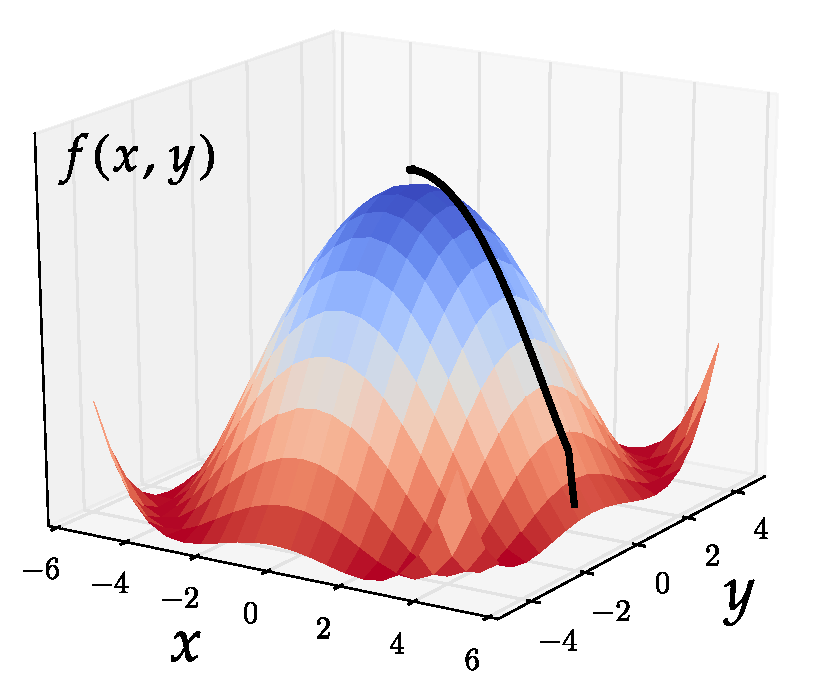
\includegraphics[width=0.7\textwidth]{figures/3dtabufunc.pdf}
  \end{figure}
  % \vspace*{-0.cm} 
\end{frame}


\begin{frame}{Exemple - Recherche tabou}


  \begin{figure}[tb]
    \centering
    Pour $f(x,y) = \dfrac{\sin(x^2+y^2)}{x^2+y^2}$
    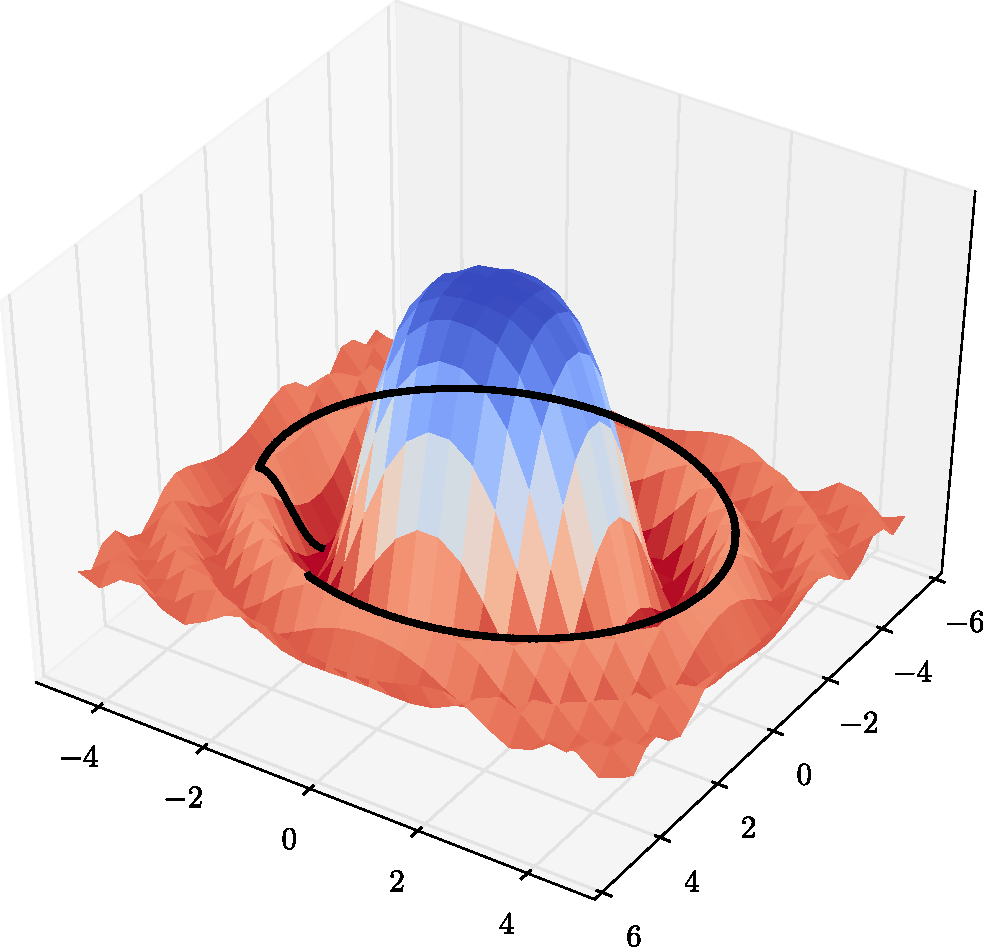
\includegraphics[width=0.6\textwidth]{figures/3dtabufunc2.pdf}
  \end{figure}
  % \vspace*{-0.cm} 
\end{frame}



\section{Algorithme des lucioles}
\begin{frame}{Algorithme des lucioles}
   \textbf{Recherche par lucioles}\\
  \textit{Type : }Métaheuristique\\
  \textit{Stochastique : } Oui\\
  \textit{Caractéristique : } Recherche globale
  \vspace{0.5cm}
  \hrule
\vspace{0.2cm}
\textbf{Principes}\\
1. Chaque luciole a une luminosité $I$ et une position.\\
2. Les lucioles sont attirées par les lucioles plus lumineuses.\\
3. L'attirance décroît lorsque la distance augmente.
\end{frame}

\begin{frame}{Exemple - Algorithme des lucioles}
  \textit{On veut aller au bas de la montagne.}
  \begin{figure}[tb]
    \centering
    \includegraphics<1>[width=0.7\textwidth]{figures/firefly1_v2.pdf}
    \includegraphics<2>[width=0.7\textwidth]{figures/firefly2_v2.pdf}
    \includegraphics<3>[width=0.7\textwidth]{figures/firefly3_v2.pdf}
  \end{figure} 
\end{frame}


\begin{frame}{Algorithme des lucioles}
  $N$ lucioles à des positions $\bm{x}_i$\\
  On optimise la fonction $f(\bm{x})$\\
  $I_i\propto f(\bm{x_i})$
  
     % $\beta_0 $: Attirance\\ $\gamma :$ Portée\\$\alpha$ : Exploration

  \vspace{0.5cm}
  \hrule 
  Si $I_j>I_i$
  \begin{align*}
    \bm{x}_i \rightarrow \bm{x}_{i} +  \highlight[myblue]{\beta_0\text{e}^{-\gamma r_{ij}^2}(\bm{x}_j-\bm{x}_i)}+ \highlight[myred]{\alpha\epsilon_i}
  \end{align*}
  $\beta_0=0$ : Marche aléatoire\\
  ($\gamma=0$ : Optimisation par essaims particulaires)
\end{frame}

% \begin{frame}{Pseudocode - Algorithme des lucioles}
%  1) Placer $N$ lucioles à différents endroits $\bm{x}_i$\\
%  2) Mesurer l'intensité des lucioles $I_i \propto f(\bm{x}_i)$\\
%  3) $\gamma$ : Coefficient d'absorption\\
%  4) $\beta_0$ : Attractivité

%  \textbf{while} (temps<temps\_max):\\
% \hspace{0.5cm} \textbf{for} $i=1..N$:\\
% \hspace{1.0cm} \textbf{for} $j=1..N$:\\
% \hspace{1.5cm} \textbf{if} $f(\bm{x}_j)>f(\bm{x}_i)$\\
% \hspace{2.0cm} Déplacer $i$ vers $j$\\
% \hspace{1.5cm} \textbf{end if}\\
% \hspace{1.cm} \textbf{end for}\\
% \hspace{0.5cm} \textbf{end for}
% Mise à jour des intensités.
% \end{frame}




\begin{frame}{Exemple - Algorithme des lucioles}
  \textit{Trouver un minimum en 2D}
   \begin{figure}[tb]
    \centering
    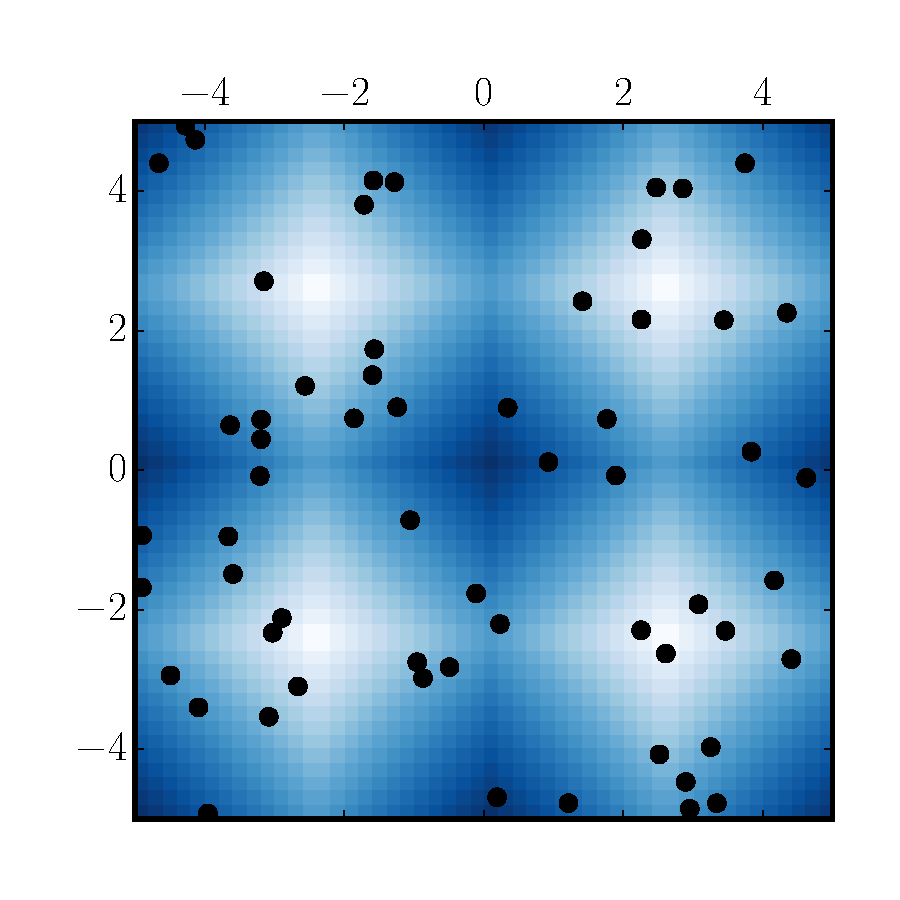
\includegraphics[width=0.49\textwidth]{figures/fireflyout1.pdf}
    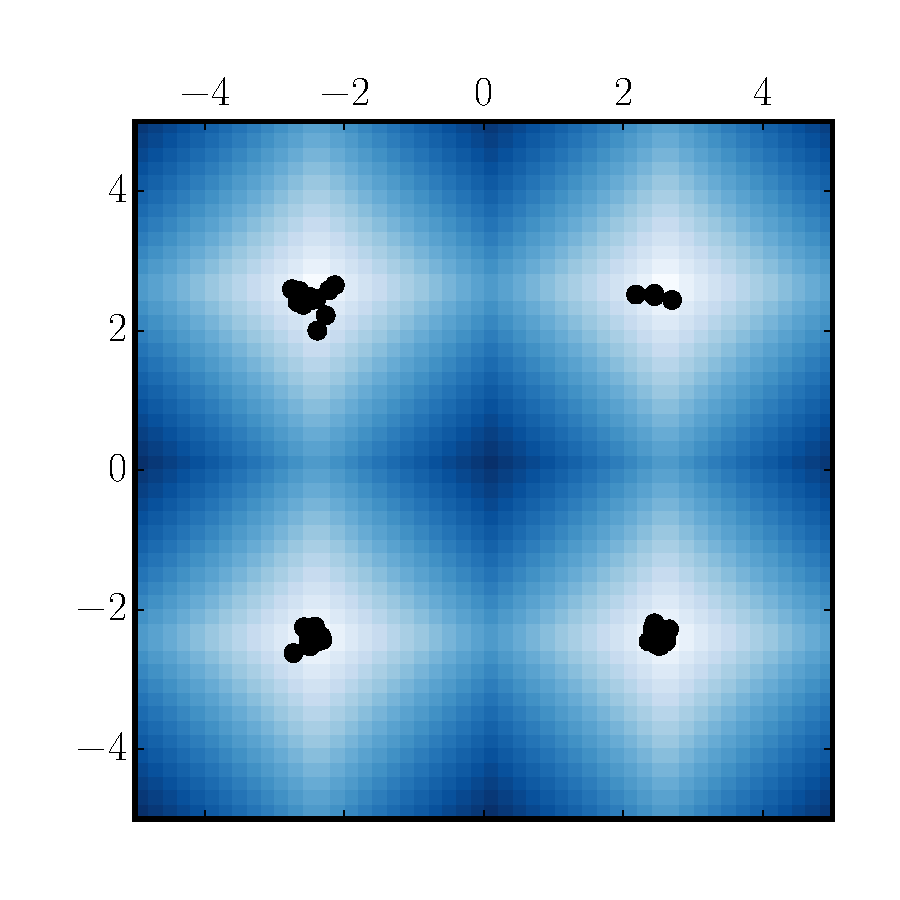
\includegraphics[width=0.49\textwidth]{figures/fireflyout2.pdf}
  \end{figure}
\end{frame}

\begin{frame}{Exemple - Algorithme des lucioles}
  Vidéo
\end{frame}

\begin{frame}{Résumé des algorithmes}
\begin{table}[h!]
  % \caption{caption here}
  % \label{tab/:tablename}
  \centering
  \begin{tabular}{ccc}
  \hline\\
  \textbf{Tabou} & \textbf{Lucioles} & \textbf{Évolutif}\\
  \hline\\

  Local & Global & Global\\\\
  Déterministe & Stochastique & Stochastique\\
    - & $\beta_0,\gamma,\alpha$ & \\
  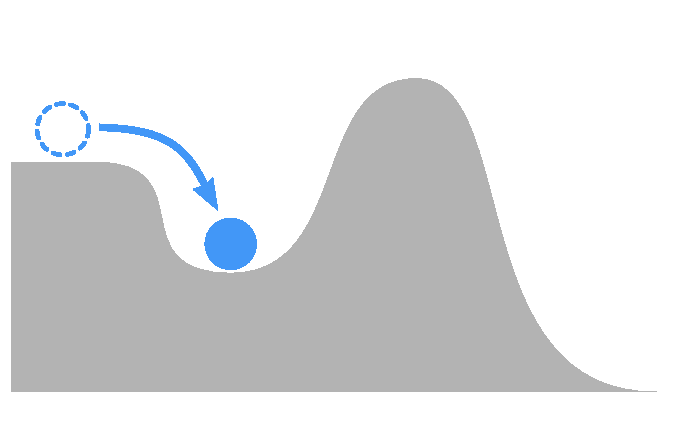
\includegraphics[width=3cm]{figures/tabou2v2.pdf}& 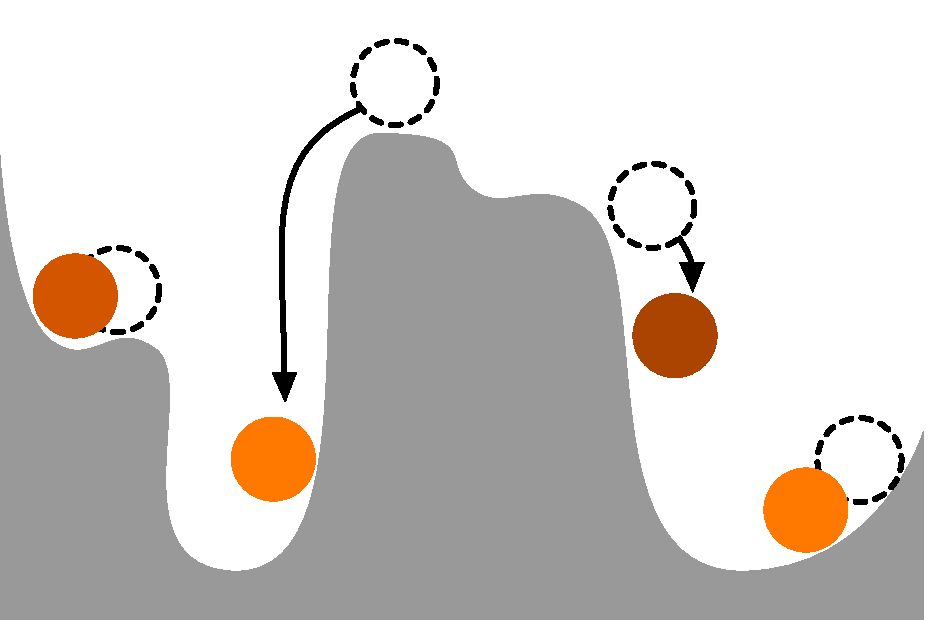
\includegraphics[width=2.7cm]{figures/firefly2_v2.pdf}\\
  \hline
  \end{tabular}
\end{table}
  
\end{frame} 


\section{Problème du vendeur}
\begin{frame}{Problème du vendeur}
  \textbf{Travelling salesman problem}\\
  Un vendeur veut visiter $N$ habitations et marcher le moins possible.\\
  \textit{Dans quel ordre doit-il visiter les $N$ maisons?}
  \begin{figure}[b]
    \centering
    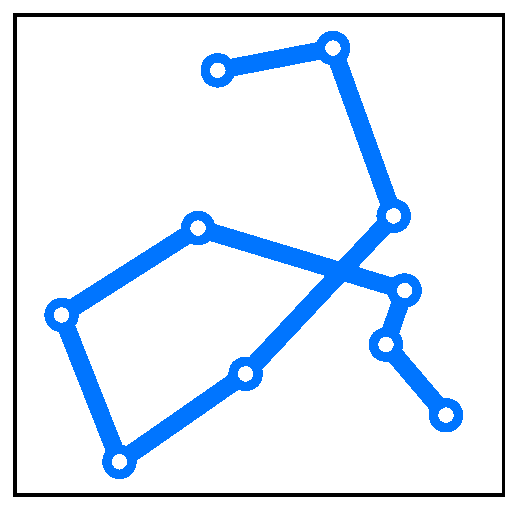
\includegraphics[width=0.28\textwidth]{figures/salesman_tabu_n10_1.pdf}
    \quad
    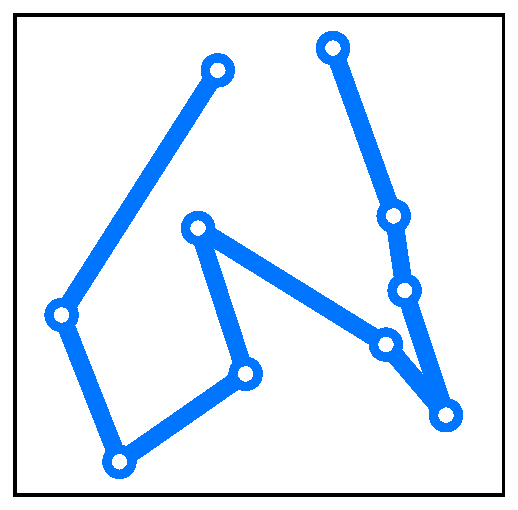
\includegraphics[width=0.28\textwidth]{figures/salesman_tabu_n10_2.pdf}
    \quad
    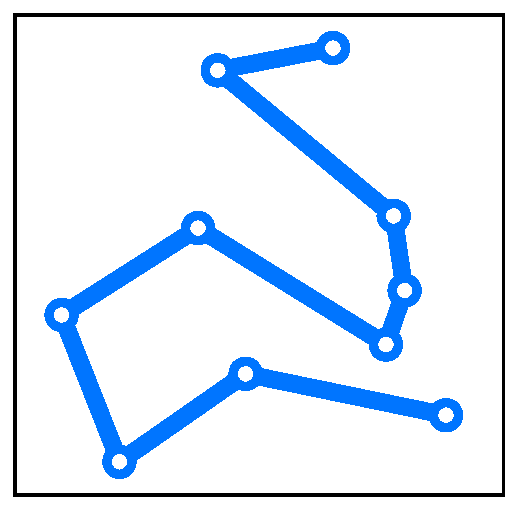
\includegraphics[width=0.28\textwidth]{figures/salesman_tabu_n10_3.pdf}
    % \caption{Caption here}
    % \label{fig:figure1}
  \end{figure}
\end{frame}

\begin{frame}{Problème du vendeur}
\begin{center}
  Meilleurs parcours pour $N=20$.
\end{center}
\vspace{-0.5cm}
\begin{table}
  \centering
  \begin{tabular}{C{3cm}C{3cm}C{3cm}}
  \textbf{Tabou} & \textbf{Lucioles} & \textbf{Évolutif}
  \end{tabular}
\end{table}
\vspace{-1cm}
\begin{figure}[h!]
  \centering
  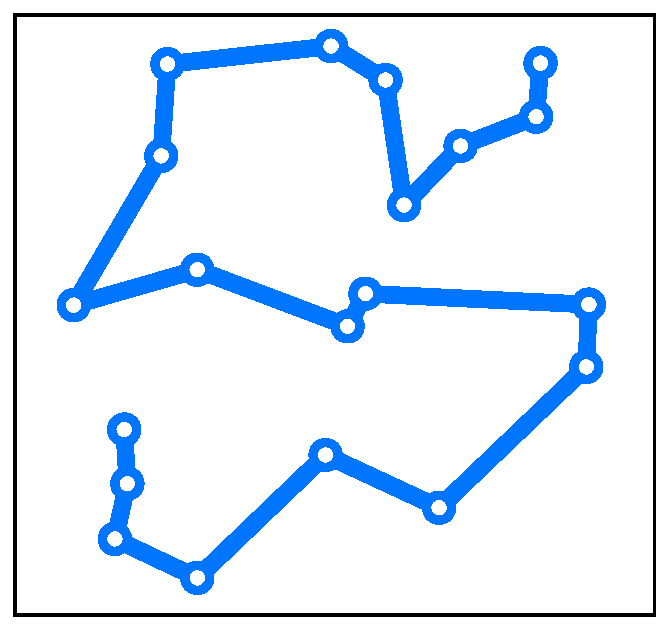
\includegraphics[width=0.32\textwidth]{figures/salesman_tabu_n20.pdf}
    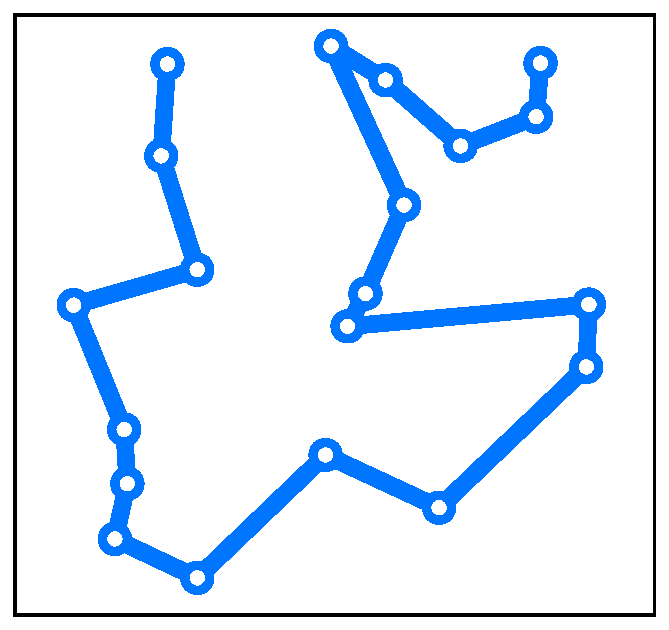
\includegraphics[width=0.32\textwidth]{figures/salesman_firefly_n20.pdf}
    % 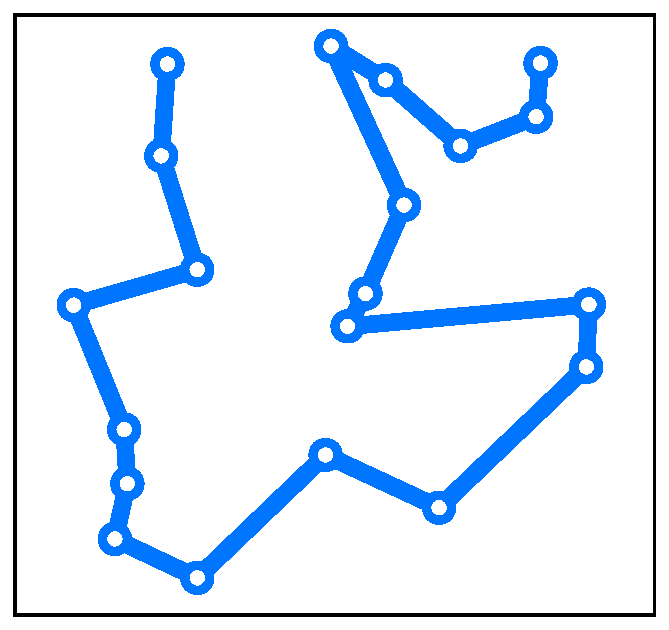
\includegraphics[width=0.32\textwidth]{figures/salesman_firefly_n20.pdf}
\end{figure}


% \begin{table}[tb]
%   \centering
%   \begin{tabular}{R{1cm}C{2cm}C{2cm}C{2cm}}
%   \hline

%   \hline
%   &\textbf{Tabou} & \textbf{Lucioles} & \textbf{Évolutif}\\
%   \hline
%   Meilleur & 35.766 & 40.171 &40.171 \\
%   Moyen & 37.293 & 42.413 &40.171\\
%   \hline
%   \end{tabular}
% \end{table}

\end{frame}



\begin{frame}{Comparaison des trois algorithmes}
  \textbf{Distribution de la qualité des solutions}
  \begin{figure}[h!]
    \centering
    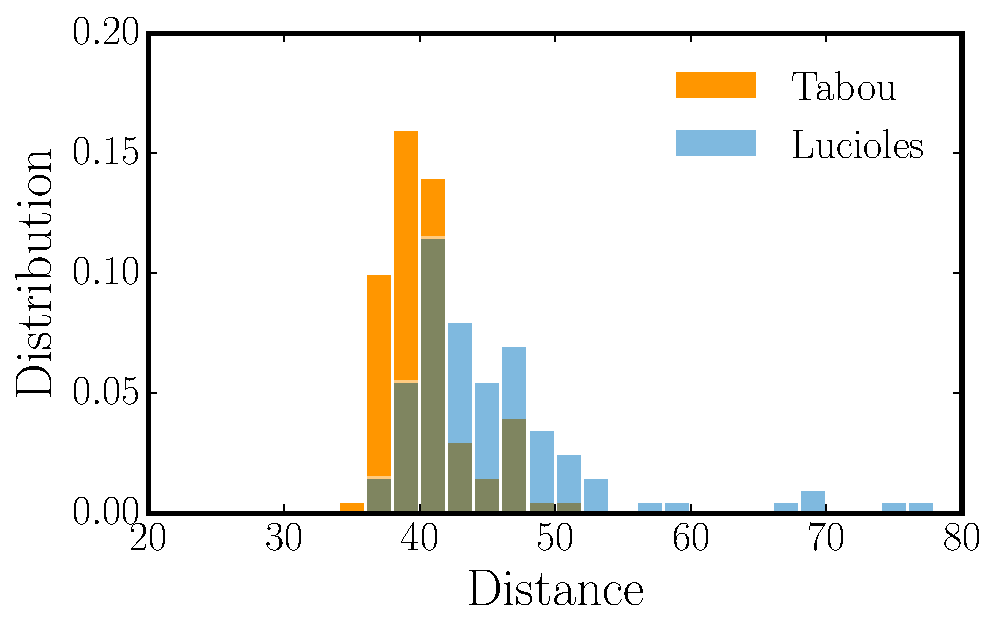
\includegraphics[width=0.85\textwidth]{figures/distri_distance.pdf}
  \end{figure}
\end{frame}

\begin{frame}{Comparaison des trois algorithmes}
  \begin{center}\textbf{Évaluation sommaire des méthodes}\end{center}
  \begin{table}
  \centering
  \begin{tabular}{C{2.6cm}C{2cm}C{2cm}C{2cm}}
  &\textbf{Tabou} & \textbf{Lucioles} & \textbf{Évolutif}\\
  \hline\\
  \textit{Qualité} & 9/10 & (7/10) &\\\\
  \textit{Vitesse de convergence} & 10/10 & (8/10) & \\\\
   \textit{Implémentation} & 10/10 & 6/10 & \\
  \end{tabular}
\end{table}
\end{frame}




\end{document}
